%\documentstyle{llncs}
%\documentclass[12pt,fullpage]{llncs}
\documentclass[12pt]{article}
%\usepackage[left=3cm,top=1.2cm,right=3cm,nohead,nofoot]{geometry}
%\usepackage[letter,left=.25in,right=.25in,top=.17in,textwidth=7.5in,textheight=9in]{geometry}
%\usepackage[left=0cm]{geometry}

%\documentclass[12pt]{report}
%\usepackage {utthesis2}              %% Preamble.

%\usepackage{amsmath}
%\usepackage{amssymb}
\usepackage{arabtex}
\usepackage{amsmath}
\usepackage{amssymb}
\usepackage{times}
\usepackage{caption}
\usepackage{epsfig}
\usepackage{subfigure}
\usepackage{color}
\usepackage{rotate}
\usepackage{rotating}
\usepackage{multirow}
%\usepackage[colorlinks=false]{color,hyperref}
\usepackage{color,hyperref}
%\usepackage{amsthm}
%\usepackage{booktabs}
\usepackage{natbib}
\bibpunct{[}{]}{,}{n}{}{;}

\usepackage{url}

\usepackage{relsize}
\usepackage{fancyvrb}
\usepackage{fancyhdr,lastpage}

\usepackage{utf8}
\setarab
\fullvocalize
\transtrue
\arabtrue

\newcommand{\CharCodeIn}[1]{`\CodeIn{#1}'}
\newcommand{\CodeIn}[1]{{\small\texttt{#1}}}
\newcommand{\frl}[1]{\fbox{\RL{#1}}} 
\newcommand{\noArRL}[1]{\arabfalse\RL{#1}\arabtrue} 
\newcommand{\noTrRL}[1]{\transfalse\RL{#1}\transtrue} 
\newcommand{\noTrNoVocRL}[1]{\novocalize\transfalse\RL{#1}\transtrue\vocalize} 
%\newcommand{\drawline}{\begin{picture}(6,.1) \put(0,0) {\line(1,0){6.25}}\end{picture}}

\usepackage{setspace}
%\doublespacing
\renewcommand{\baselinestretch}{1.15}
\setlength{\parindent}{0in}
%\parskip 6pt
%\parindent 0pt
%\setlength{\parskip}{.05in}
%\oddsidemargin 0in
%\evensidemargin 0in
\oddsidemargin .0in
\evensidemargin .0in
\hoffset -.75in
\voffset -.83in
\textwidth 7.5in
\textheight 9.5in

\topsep 0in
\topmargin 0.17in

%\usepackage{arabtex}
%\usepackage{utf8}

\begin{document}


\pagestyle{fancy}
%\lhead{}
\chead{}
\rhead{NPRP No.~:~~~~4-484-1-075}

\lfoot{QNRF Form}
\cfoot{}
\rfoot{Page \thepage~of~\pageref{LastPage} }
\renewcommand{\footrulewidth}{0.2pt}
\renewcommand{\headrulewidth}{0.2pt}

%\begin{titlepage}

\begin{center}
{\Large \bf Relational Arabic Text Mining Framework using 
    Morphological
    and Case-Based Analysis }

%\setlength{\unitlength}{1in}
%\setlength{\unitlength}{1in}
\vspace{1.5in}

\renewcommand{\arraystretch}{.6}
\begin{tabular}{cc}
Fadi Zaraket & Rehab Duwairi \\
Electrical and Computer Engineering &  Computer Science and Engineering Department \\
American University of Beirut & University of Qatar \\
{\tt fadi.zaraket@aub.edu.lb} & {\tt Rehab.Duwairi@qu.edu.qa}
\end{tabular}

\vspace{1.5in}

\renewcommand{\arraystretch}{.6}
\begin{tabular}{c}
{\small Research Plan Document } \\
{\small Proposal Submitted to }\\
\\
    Qatar National Research Foundation \\
    National Priorities Research Program \\
    4$^{th}$ Cycle 
\end{tabular}
\vspace{.5in}

\date{\today}
\pagebreak

\end{center}

\section{Background (max of 2 pages)}
\label{s:background}

Research in text mining started in the mid 1980s when Swanson 
realized that slicing and combining seemingly unrelated medical 
articles led to the discovery of new 
hypotheses~\cite{JNi06}.
Till present, most of the interest in text mining comes 
from biological sciences.
Lately we saw applications of text mining in the advertisement, 
political campaigning, and other businesses.
Text mining involves information retrieval (IR), natural language 
processing (NLP), information extraction (IE), 
and data mining~\cite{ASr09}.

Most of academic research in the field of Arabic text mining 
is covered in the almost comprehensive book 
``Arabic Computational Morphology''~\cite{Sou07}.
The book summarizes recent work, and presents strong evidence of 
shortage of historic research. It also highlights  an emerging 
interest in this area with a specific application to machine 
translation from Arabic to English after 2001.
The research community showed little interest in 
automating Arabic text analysis that may serve
the Arabic user.
While a non-Arabic user is interested in machine translation to 
help him understand an Arabic document, 
an Arabic user is more interested in 
information hard to discover manually such as 
the relation between clinical records, pharmaceutical 
prescriptions and sales, and a specific sickness. 
Another Arabic user may be interested in looking at the relation
between stock prices and political news or the 
relation between suspect profiles in interrogation reports 
and investigative reports from the crime scenes. 

We propose to build a 
%{\em relational text mining 
%of Arabic using morphological and case-based analysis}. 
{\em case-based Arabic text analysis using relations and morphology}(CATARM) framework. 
CATARM will take as input sets of documents, each of a specific
type, and provides the user with a visual query language that
allows him to build a flow of Arabic text mining
modules and discover desired relations between documents. 
CATARM will translate the query into a netlist of computational 
components, it will also extract parameters from the query and 
the document sets and use them to simplify the computational 
components. 
%The main CATRAM computational components will be finite 
%state machines (FSM) that express a linguistic model of the Arabic 
%language and that can be parametrized and relaxed to fit a case 
%study. 

%IR tools are similar to a Google search 
%engine where documents of interest are selected based on the 
%relevance to a set of keywords of interest to the user.
%NLP targets the automation of understanding human languages.
%This task is the oldest and most difficult task in the artificial 
%intelligence domain.
%The main difficulty behind NLP comes from the ambiguity of 
%natural languages~\cite{Osm08}.
%While NLP techniques cannot deliver their final target yet, they 
%can deliver analysis of sentences into nouns, verbs, and adjectives.
%They can also narrow the meaning of a word or a phrase based on 
%the context to one of its possible meanings.
%Finally they can parse a sentence into a relation between the 
%discovered entities using abstractions such as verb-name 
%abstractions~\cite{Osm08}.

%Information extraction (IE) targets forming data structures and 
%instances of these data structures out of a collection of documents.
%IE tries to fit the output of IR and NLP to templates of 
%interest to the user.
%Data mining can be applied at the end on the output of the 
%IE process to answer user queries about the input 
%documents~\cite{JHa05}.

%\subsection{Arabic text mining in academy }
%In the following we review the major works on Arabic text mining 
%in academy and industry.

Arabic morphological analyzers~\cite{Sughaiyer:04}
consider an Arabic word and its internal structure composed of 
several {\em morphemes}. 
A morpheme is a {\em stem} or an {\em affix}.
An affix is a {\em prefix, suffix,} or an {\em infix}.
The analysis of one word may lead to several possible
solutions.
\vocalize
For instance, the word 
\RL{'a.hmadH}~\footnote{In this document, we use the default 
ArabTeX transliteration style ZDMG.}
may have two valid morphological analyses. 
The word means ``I praise him'' when
the letter \RL{'a} is a prefix and  it means
``his Ahmad'' when 
the letter \RL{'a} is part of the proper noun stem 
\RL{'a.hmad}.
\novocalize

%The accuracy of the solutions suffer due to inherent difficulties
%of morphological analysis of the Arabic language. 
It is common practice to write Arabic text
without short vowels. 
This greatly increases the ambiguity of Arabic text. 
Arabic letters can have up to 
four different forms
corresponding to their position in a word, i.e, beginning,
middle, end of word and separate forms. 
This allows the phrase
\noTrRL{il_A\nospace almdrsT}  with no delimiter within
to be visually recognizable
as two separate words \RL{il_A} (to) and \RL{almdrsT} (the school).
This happens because the first word \RL{almdrsT} ends with
\RL{T} a non-connecting letter. 
These words occur often in text and greatly increase the
difficulty of tokenization and are referred to as 
``run-on'' words~\cite{Buckwalter:04}.
Such difficulties are inherrent to the 
morphological analysis of the Arabic language and
render the solutions inaccurate.

Current morphological analyzers such as 
Buckwalter~\cite{Buckwalter:02},
Beesly~\cite{Beesley:01}, SAMA~\cite{Kulick:10},
and ElixirFM~\cite{Otakar:07} exist.
These analyzers are used in several open source spell checkers as 
well as NLP frameworks~\cite{Col09}.
They take as input white space delimited tokens~\cite{Kulick:10},
consider them as words,
and enumerate all possible solutions. 
This approach has several problems. 
First, a white space delimited token may have 
more than one word.
Second, the exhaustive enumeration may hurt performance and may
not be necessary or appropriate
in some case studies~\cite{Maamouri:10}. 
Other morphological analyzers such as 
Amira~\cite{Diab:07,Benajiba:07},
MAGEAD~\cite{Habash:05}, and MADA+TOKAN~\cite{Habash:09} 
use machine learning and support vector machines (SVM) 
to enhance the accuracy at the expense of efficiency.

{\bf Hypothesis 1.} We hypothesize that many case studies, 
in particular relational
case studies, do not require high accuracy from the 
low level morphological analysis.
The sophistication of the sought higher level query can eliminate 
many of the ambiguous low level solutions at a lower computational 
cost.
For example, if a query concerns proper names and the 
prefix in question in the analysis connects only to a verb, 
we do not need to further analyze the rest of the word 
to provide an answer.

We find evidence to our hypothesis in~\cite{Maamouri:10}. The 
addition of a new corpus to the Arabic Tree Bank~\cite{Maamouri:04}
required the high NLP task to interact with the low 
level morphological analyzer.
This led to a refined analyzer~\cite{Kulick:10}.  
We also find evidence in~\cite{Habash:06} that different types of 
morphological analyses behave differently on the same case study. 
We strongly believe and we find evidence in our preliminary
results that a 
case-based morphological analyzer that allows a high level 
case-based controller to intervene at every decision to 
guide, use, prune, and refine the morphological analysis
is of high utility.

%Prior work in Arabic text mining addressed the classification and 
%categorization of Arabic text and made little use of features 
%unique to the Arabic language.
Researchers in~\cite{AEL07,Ham07,Abd07,MEl03} 
preprocessed the Arabic text to make it presentable to known text 
mining techniques that tend to Latin text and queries.
%Buckwalter~\cite{Bee89,Tim04} uses morphological analysis to enable 
%relaxed stemming of Arabic words.
El-Halees used statistical analysis to address the problem of 
classifying Arabic text documents with maximum 
entropy~\cite{AEL07}.
In~\cite{Abd07} Mesleh evaluated six different techniques to 
classify Arabic text using a support vector machine.
El Dost~\cite{MEl03} used root words in the Arabic language to 
speed up automated and hierarchical indexing.
Al-Zoghby~\cite{Ham07}
%addresses the problem of 
%entities extracted from Arabic text with similar content but 
%slightly different names via 
used the derivation feature in 
the Arabic language as a similarity measurement.
This work is limited to the names of the fields in the data 
structures extracted from Arabic texts.

{\bf Hypothesis 2.} This approach does not tend directly to 
the Arabic users who write their 
queries in Arabic and think in Arabic.
We hypothesize that Arabic queries use rules and 
relations similar to the Arabic text under investigation, 
and thus techniques native to the Arabic language will do better 
in Arabic text analysis.

We find evidence in the work of the CADIM \noTrRL{q-adim} 
project~\cite{Col09} at the University of Columbia to support our 
hypothesis. They observe that Arabic texts used as training 
data for common NLP techniques proved ineffective. 
They built semi-automatic models to address the problem of automatic 
speech recognition in Arabic.


%\subsection{\bf Arabic text mining in industry}
Few companies in the industry provide primitive Arabic text 
analysis tools.
Sakhr~\cite{Sak09} provides a categorization 
tool with a limited number of predefined categories, and a summary 
generator that selects sentences from text.
Basis technology~\cite{Bas09} provides Rosette, a lexical 
analysis tool that normalizes Arabic text as a pre-processing step 
for indexers and other general purpose data mining 
tools.  Basis also provides REX; an entity extractor.

ElixirFM~\cite{Otakar:07} uses an {\em inferential-realizational}
approach for morphological analysis. 
Realizational morphology considers the form of the word 
\noTrRL{.sarf}  instead of its segments. 
Formal rules and formulas express the relations between 
the root of the lexeme and the fully inflected word. 
While this is highly compatible with the Arabic linguistic 
description~\cite{Badawi:04},
and it benefits from features unique to the Arabic language
captured by the formal rules, 
it is computationally expensive and enumerates all the possible
solutions. 

{\bf Goals.} Up to our knowledge, CATARM will be the 
first framework that tends to relational Arabic morphology 
and text mining. 
{\bf (1.)} CATARM will build a novel parametrized linguistic 
computational model of Arabic. 
The model will be implemented using efficient structures. 
 {\bf (2.)} It will be amenable to Arabic specific simplifications 
inferred from the correspondence between the fromal Arabic rules
and the relational user queries.
{\bf (3.)} The model will also be amenable to simplifications 
inferred from statistical features extracted from the document 
sets using language independent techniques such as latent semantic 
indexing~\cite{LSI89} and hidden Markov models (HMM).
%CATARM will augment current digital dictionaries to resolve 
%entity semantics and targeted qualificationsl.
{\bf (4.)} CATARM extracts semantic graphs from each text 
document and then uses set arithmetic and graph analysis techniques
to establish relations between these graphs. {\bf (5.)} CATARM will 
solve at least three interesting relational Arabic text case studies 
presented in Section~\ref{s:design:casestudies}.

\pagebreak

\section{Objectives and significance (max of 1 page) } 
\label{s:objectives}

The current prevailing direction in research 
in Arabic text mining and NLP focuses on machine translation from 
Arabic to English. 
A little attention is given to native Arabic text mining 
problems and applications. 
CATARM is a relational Arabic text mining 
framework that tends to Arabic users 
with the following objectives.

\begin{itemize}\itemsep0pt
\item CATARM will build a formal Arabic computational model
using efficient and configurable data structures such as 
finite state machines (FSM). 
\item CATARM will provide the user with a visual query 
language that makes it easy to enter relational queries. 
The query language will also allow the framework to extract Arabic
specific features from the query to simplify the linguistic 
computational model. 
\item CATARM will use statistical models and techniques
to infer language independent features from the text documents
that will further simplify the computational model. 
\item During the project, we will augment current Arabic digital 
dictionaries to resolve entity semantics and targeted 
qualifications such as adjectives.
\item The framework will allow the integration of library and 
custom computational components built on top of primitive
CATARM components. 
The components will be the linguistic computational model,
statistical, set arithmetic, logic,
and graph analysis techniques, and  text algorithms.
\item We will use CATARM to solve several realistic case studies.
We will look at the hadith literature and build a system using
CATARM to relate the hadith literature to the biographies of the
narrators and extract an authenticity graph for the narrators.
We will look at investigation and interrogation security reports
and build a CATARM system that looks for relations between suspects
in the reports. 
We will look at clinical reports and relate them to pharmaceutical 
records and find relations between sicknesses and prescribed medication. 
Finally, we will build a system using CATARM to check the strength
of the relations between internet documents viewed by a minor and
a set of Arabic text documents containing unrated or unwanted 
material. If the relation is strong, the system will flag access to
the document. 
All components and parts built during the development of solutions
to the case studies will be generalized and added to CATARM as 
library computational components. 
\end{itemize}


%\begin{itemize}\itemsep0pt
%\item {\bf The literature case study.}
%We are given a set of books of historical accounts where
%a chain of narrators precedes each account,
%and a second set of books of biographies where
%a biography includes an evaluation of the authenticity 
%of the narrator therein.
%CATARM will allow the user to automatically and exhaustively query 
%all accounts related to a subject important to Islamic jurispudence 
%(for example women and travel),
%and extract a graph where nodes represent narrators and edges
%are labeled with the authenticity of the narrators. 
%A similar manual query takes ages to answer and is error prone.
%\item {\bf The security case study.}
%Given two sets of reports consisting of crime scene investigation 
%and suspect interrogation reports, 
%an officer may query CATARM 
%for relations between suspects in terms of 
%criminal action, locality, or third party persons unknown to the 
%officer.
%Such a query is very hard to answer manually.
%\item {\bf The net traffic case study.}
%Given a set of undesired internet content for minors
%such as violent text, and a set of documents requested by internet
%minor users, 
%CATARM can discover whether there is a relation between 
%the document and the violent content and flag the document if the
%relation is strong enough. 
%\end{itemize}
 
\subsection{Significance} 

CATARM will discover relations between Arabic text documents that 
are hard to discover by humans and will have direct live and
cost saving benefits in cases similar to the above mentioned 
case studies. 
CATARM will qualitatively enhance research in the cultural and 
literature fields. 
It may also help investors analyze Arabic news and data from Arab 
markets prior to making important decisions.

The use of Arabic text mining  will 
have a high impact on the prosperity and safety of the Arab world 
in particular and the world in general.
%For example, having the tools to check the authenticity of a hadith 
%at a click of a button may save youth from the hands of extreme 
%religious leaders.
For example, extracting a relation between two criminals may 
uncover a third criminal who is ready to commit a crime.
Finding inconsistencies in claims may curb down fraud and corruption 
in the insurance sector.

In addition, building the necessary academic 
infrastructure for Arabic text mining in Lebanon and Qatar will 
open the way for investments in the field and provide work 
opportunities for native workers.

\pagebreak

\section{Preliminary data or studies}
\label{s:prelim}

The PI and his team at the American University of Beirut (AUB)
started work on an Arabic text mining framework~\cite{ATMine09}
that is available now online.
They have successfully developped ATSarf, a case-based morphological 
analyzer, and applied it on the hadith literature case study. 

A \RL{.hady_t} is a narration related to the prophet Mohammad
through a \RL{sanad} or a sequence of narrators. 
Figure~\ref{f:exhadith} shows an example \noArRL{.hady_t} in Arabic with its 
transliteration and translation. 
The authentication of a \noArRL{.hady_t} highly depends on the credibility
of each of the narrators as reported in separate biography 
books. 
We consider the problem of automatically segmenting
a \noArRL{.hady_t} book into narrations, then segmenting each 
narration into
its content or \RL{matn} and its \noArRL{sanad} or the
chain of narrators.
We also partition the sanad accurately into the 
separate narrators so that we can later look each one of them 
up in the biography books. 
For example, the boxes in Figure~\ref{f:exhadith} are proper names 
and once
connected toghether they form complex names of narrators. 
Narrator $n_1$ has the first name \noTrRL{qtybT} and his father 
name is \noTrRL{s`yd} as the word in between 
\noTrRL{bn} (son of) indicates. 

\transfalse
\begin{figure}[tb]
\center{
\resizebox{.7\columnwidth}{!}
{ \input{figs/exhadith.pdftex_t}}
\caption{Hadith abstraction example.}
\label{f:exhadith}
}
\end{figure}
\transtrue

The framework now comprises a state of the art
case-based morphological analyzer, ATSarf, 
and computational components that allow the user to
specify his queries as one or more FSM
controlling the morphological analyser.
We explain this approach in details in Section~\ref{s:design:fsm}.
ATSarf along with other computational components, 
extract the chains of narrators from a set of narrations
with above 95 percent accuracy and in less than two minutes. 

\begin{figure}[tb]
\center{
\resizebox{.75\columnwidth}{!}
{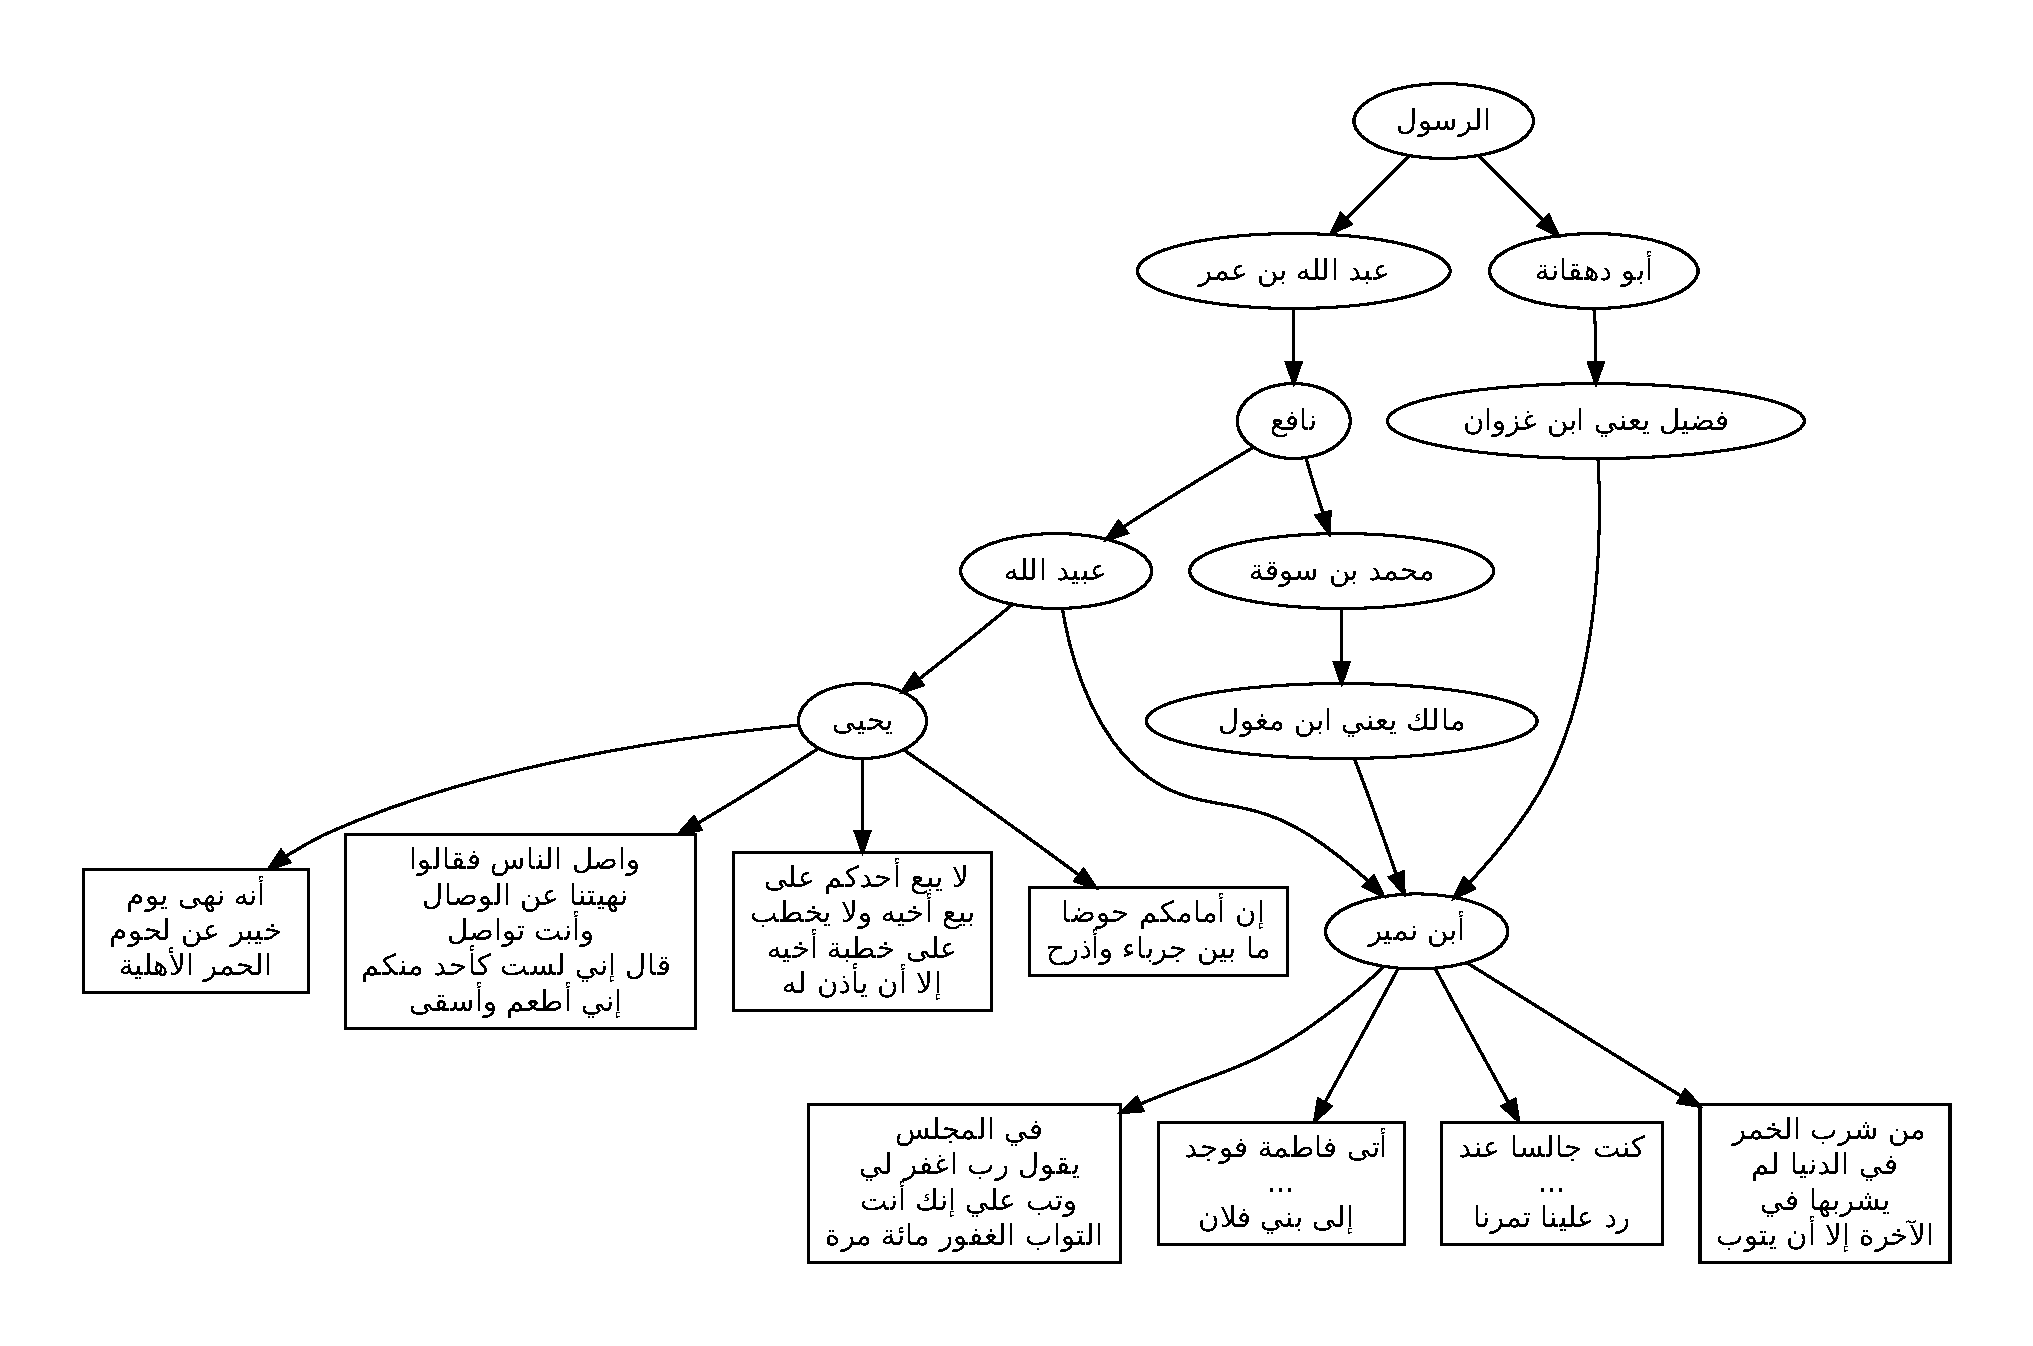
\includegraphics{figs/narrator_chain_output.pdf}
\label{f:narrators} } 
\caption{Directed acyclic graph representing a partial order 
    relation between narrators extracted using ATSarf}
}
\end{figure}

The directed acyclic graph (DAG) 
in Figure~\ref{f:narrators} shows a partial order relation (POR) between
narrators.
We automatically extracted the POR from hadith text 
documents.
The nodes in boxes are the \RL{matn} of the hadith, 
and the other nodes are the narrators.
Given a set of chains of narrators similar to 
Figure~\ref{f:exhadith} we formed the DAG using graph algorithms 
that merged equal names in the chains. 
This partial order graph is instrumental to automate
localizing narrators in biography documents and
segmenting biography documents.

Given that a biography will discuss a narrator and mention
his professors and students,
we can segment the biographies with a graph coloring algorithm 
that traverses the text and colors the POR whenever
a name is found. 
We modify the color when we move in the graph 
far away from the last name we colored.

Once the biographies are analyzed, one can annotate
the POR with qualifiers of the narrators that reflect
their authenticity. 
One can also annotate the POR with the locations and 
the time they lived in. 
Then One can compute a time and location overlap
check to discover inconsistent narrations.
We can also perform several interesting checks using 
this POR on its own such as checking for the effect of
one narrator on the hadith literature. 

We think that the ability to extract such orders
between entities in documents can 



These preliminary results serve as a good proof of concept to our 
hypothesis. They also confirm that our approach performs better than 
currently existing techniques from Sakhr~\cite{Sak09},
Basis~\cite{Bas09} and open source 
tools~\cite{Col09,Otakar:07,Tim04}.

We find evidence in our current results that features 
of the Arabic language such as the hierarchical structure of
names can be used to simplify the morphological analysis
needed to extract the partial order graph. 
Publications about these results are pending acceptance in 
related NLP conferences. 

The Co-Lead PI published extensively in this domain. 
A selected list of her recent publications follows. 
\begin{itemize}\itemsep0pt
\item Rehab Duwairi, Mohammad Al-Refai, Natheer Khasawneh, 
"Feature Reduction Techniques for Arabic Text Categorization". 
Journal of the American Society for Information Science and Technology 
(JASIST), Volume 60, Issue 11, pages: 2347-2352, 2009. 
\item Rehab M. Duwairi, "Arabic Text Categorization", 
International Arab Journal for Information Technology (IAJIT), 
Volume 4, Number 2, pages 125  132, 2007.
\item Rehab M. Duwairi, "Machine Learning for Arabic Text Categorization". 
Journal of the American Society for Information Science and Technology 
(JASIST), Vol. 57, Issue 8, pages 1005-1010, 2006.
\end{itemize}


%The Lead PI worked in the area of software arabization since 1996 
%as he worked on developing Arabization modules for Windows NT and 
%an 
%Arabic string manipulation library~\cite{Zar96}. 
%The Lead PI is also involved in working on an open source 
%project that aims at comprehensive automation of authenticity 
%checks against a corpus of literature heritage~\cite{Zaraket06}.
%The Lead PI is leading an effort at AUB to introduce 
%Computational Arabic in the curriculum of the ECE program. 
%He is also leading a team of students in an effort to place 
%the infrastructure needed for this project to start. 
%The lead PI worked and published about relational logic and 
%logic solvers applied to structured languages as follows.
%\begin{itemize}
%\item Sequential circuits for relational analysis. F. Zaraket, A. Aziz, and S. Khurshid. International Conference on Software Engineering, Minneapolis MN, 2007. 
%\item Sequential circuits for program analysis. F. Zaraket, A. Aziz, and S. Khurshid. Automated Software Engineering, Atlanta GA, 2007. 
%\end{itemize}

\section{Research design and methods}
\label{s:designmethods}

%\begin{figure}[tb]
\begin{figure}
\center{
\resizebox{.75\columnwidth}{!}
{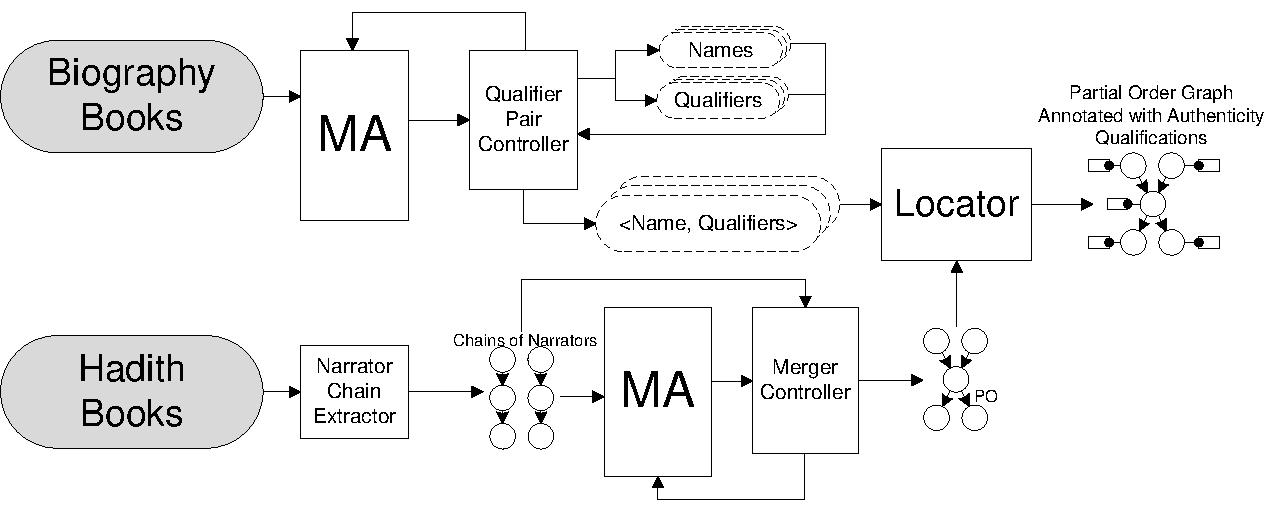
\includegraphics{figs/literature_case-study1.pdf}
\label{f:literature}
} 
\caption{CATARM diagram for the literature case study }
}
\end{figure}

%\begin{figure}[tb]
\begin{figure}
\center{
\resizebox{.8\columnwidth}{!}
{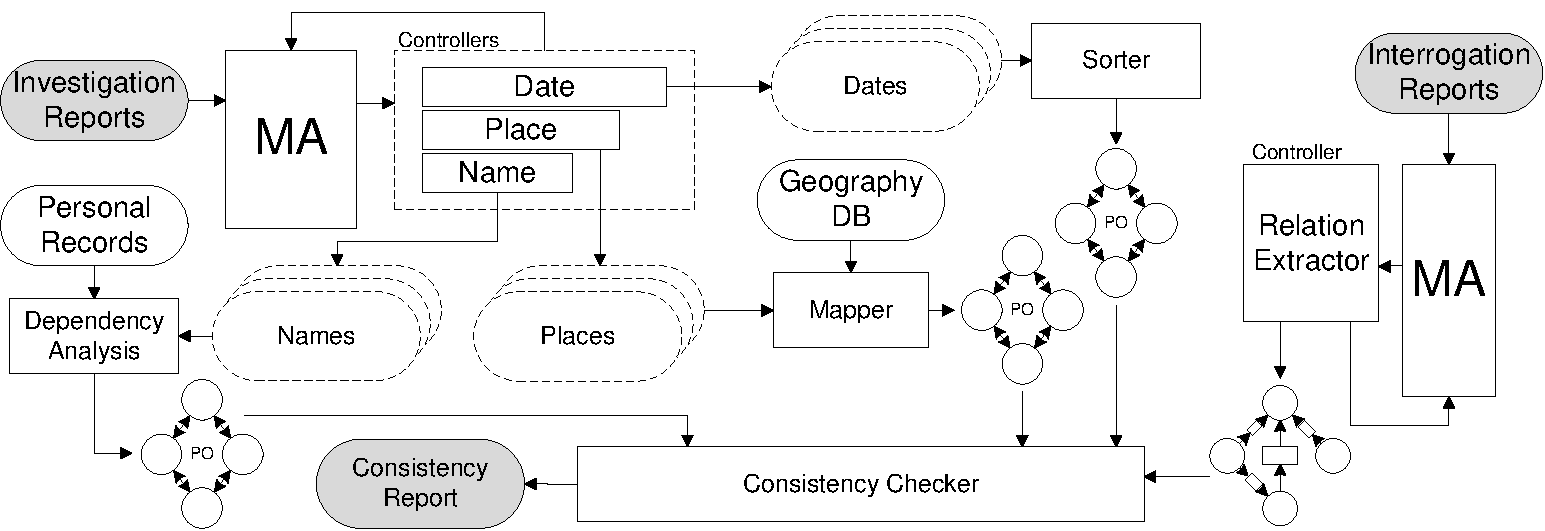
\includegraphics{figs/security_case-study.pdf}
\label{f:security}
}
\caption{CATARM diagram for the security case study}
}
\end{figure}



%\drawline
%\begin{figure}[tb]
\begin{figure}
\center{
\resizebox{.8\columnwidth}{!}
{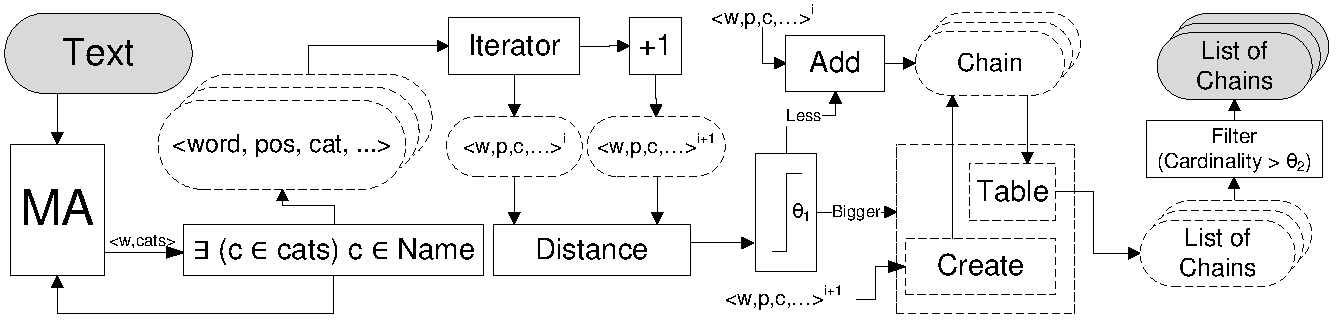
\includegraphics{figs/detailed_submachine.pdf}
\label{f:chain}
}
\caption{CATARM detailed diagram for the chain of narrators extractor}
}
\end{figure}
Consider Figure~\ref{f:chain}, which depicts a possible rendering of a query that transforms a hadith text file into a list of chain of narrators. Note that this diagram does not faithfully translate the state machine we are currently implementing to generate our priliminary results which is represented in  Figure~\ref{f:statemachine}. Instead, it has been simplified in order not to clotter the diagram. We start first by defining the legend: we have used boxes to represent computational blocks provided by CATARM, while ovals represent structured or unstructured data which are mainly the inputs and the outputs of the computational blocks. When the data blocks are dotted they represent temporary values, while when they are solid and shaded they represent the initial input and the final output. When a data block represents an array of values, the oval will be reproduced three times to show that multiple values exist.


This query generates the list of chains by first passing the hadith book text file into a Morphological analyzer which is controlled by an entity extraction controller which in this case detects Names (of people) and output such a word, its corresponding position in the text and its syntax category which must be a Name category. Then we "Iterate" over this list compoputing the distance between the positions of 2 consecutive words. This distance is inputed into a thresholding block which returns the appropriate values for the "Less" and "Bigger" outputs. Having "Less" as TRUE, means that the distance is less than the provided threshold $\theta_1$ (which is a modifiable parameter of the block). In that case, we add the word to a temporary data block representing a chain (i.e. a list of narrator names). Otherwise, we execute a sequential block which in order contains: (1) a "Table" block which tabulates the chain into a temporary table/array containing the list of chains. (2) a "Create" block which initializes a new "Chain" whith the output of the second iterator (i.e. the name whose distance from its previous one is larger than the threshold). Finally, the "Filter" block outputs only the chains whose cardinality is larger than some threshold  $\theta_2$.


In this way, the above query adds names to the chain temporary variable until a name which is distant is detected. Then, we consider the valid chains as those which contain a minimum number of names. CATARM allows the librarization of this query into a user-defined computational block that can be used later in more complex queries as will be shown below. Thus, the details of the implementation of the block will be hidden and the block's interface will be only the shaded data blocks in the figure. In what follows, we assume that this query has been librarized into a "Narrator Chain Extractor" computational block to be used in Figure~\ref{f:literature}.

\begin{figure}
\center{
\resizebox{.4\columnwidth}{!}
{\input{figs/hadith.pdftex_t}
\label{f:statemachine}
}
\caption{State-machine used to detect the chain of narrators}
}
\end{figure}

\pagebreak


%\drawline
We see more and more Arabic documents such as texts,
books, publications, hospital and governmental records emerging 
every day.
Most of the newly generated documents are produced in digital 
textual form while also old paper documents are ported to digital 
form.
These documents include huge amounts of information that is 
qualitatively different than structured information such as that 
contained in database entries.
Text mining is the technology that automates the discovery of 
information in non structured text.

Text mining concerns the partitioning of text segments into classes,
the clustering of text segments,
the extraction of concepts and entities from text,
and the discovery and modeling of relations between text entities 
and classes.
Text mining techniques perform NLP to analyze text and perform 
IE to extract information into data structures.
Fundamental to IE are the named entity (NE) and the named entity 
relation (NER) extraction techniques which capture features from 
sentences and phrases.
A key challenge to NE and NER is that sentence structures and 
words are often ambiguous in natural languages.
%While research to address ambiguity in Latin languages is still 
%lagging behind~\cite{Red08},
%not much has been done to address NE and NER in the context of 
%the Arabic language.

The application of text mining techniques to Arabic text documents 
will result in great benefits to many research fields such as 
Arabic literature,
Islamic studies, Hadith authentication, and Arabic history and 
culture in general.
Arabic text mining will also benefit sectors where Arabic text 
documents are key such as the security sector,
the government personal records,
the taxation department,
the health sector,
as well as the trading floor of a stock exchange.
 
The difficulty of applying text mining techniques to Arabic text 
documents lays in the absence of automated tools that understand 
the unique features of the Arabic language.
%We will make use of an example to illustrate the process.
Given an Arabic text document we want a tool that can segment 
and isolate all names, dates, time of the day occurrences,
tool names, and locations as entities.
Then we want another tool to identify relations amongst 
these entities such as identities and orders.
An order between two entities can be simply 
their order of appearance in the document, or their
numerical 
 We want another tool to look at the verbs and actions in the sentences and try to build relations between the identified entities based on these verbs.
 If we were successful to do that,
 we now want to order all entities associated with dates based on a chronological order.

To do the above,
 we need tools that are able to automatically differentiate between names,
 verbs,
 adjectives and other vocabulary structures.
 This is not a simple task with the Arabic language.
 For example,
 Arabic grammar allows name-based sentences or sentences with no 
    verbs \noTrNoVocRL{^gml ismiyT} .
 Another unique feature is the possibility to have names in Arabic 
 that express action such as noun verbs 
 \noTrNoVocRL{ism f`l, f-a`l $\ldots$}.

 In addition to these structural differences,
 there are features in the Arabic language that need special 
 treatment such as derivatives and stems 
 \noTrNoVocRL{alm^staq-at w al^g_dwr}.
 We also need to build dictionary tools that associate words and phrases based on their meanings and their context.
 Often time,
 and depending on the application and the user of the tool,
 we need to allow the user to assign meanings and semantics for patterns in the text.

In the following we discuss our research methodology to develop the proposed Arabic text analysis tools.
 
Lexical analysis library: We need a library of routines that enables primitive lexical analysis of Arabic text.
 For example,
 simple primitive tasks such as comparing two strings need special attention in Arabic since each Arabic letter has four different forms depending on its position in the word; isolated form,
 start,
 middle and end of a word.
 Arabic diacritics should also be ignored most of the time when comparing two strings.
 These lexical analysis routines should also pay attention to the form of a letter when used in tokenization as a letter in and end of word form denotes the end of the word even if it was not followed with a space.
 Such a library can benefit from existing Unicode enabled string libraries such as Qt.
 It also can provide a layer of abstraction that hides the details of the encoding of Arabic letters used in the text documents.
 
Syntax analysis library: This library should allow sentence structure understanding.
 We will explore the best way to develop this library.
 Several options exist such as pattern based matching,
 tokenization and dictionary based lookups,
 or a language grammar that allows more than one matching rule.
 This library needs to be extendible to allow additions of new rules or patterns.

 (Note the ElixirFM does this)
 We will explore Arabic grammar books such as The Principles of Arabic~\cite{Sha73} and others~\cite{Abd00,Abd001}
 to augment current morphological analyzers~\cite{Tim04} and syntax analysis tools~\cite{Col09}.
 We will use relaxed NLP techniques to overapproximate results.
 Then and after a relational query,
 we will apply statistical analysis techniques to rank the matching results.

Dynamic modern Arabic dictionary: The dictionary will allow identities based on semantics,
 derivation rules,
 as well as user assigned rules.
 The dictionary will return modern grammatical categories for words classifying them as nouns,
 verbs,
 and adjectives instead of the classical Arabic categories that specify how the word is derived from an original radix.
 It remains to be explored how to represent these categories without exploding the size of the dictionaries with redundant words of multiple categories.
 This work will augment existing open source Arabic dictionaries and will allow for better morphological analysis and entity extraction.

An entity extraction library: We will explore building a library that allows extraction of entities from Arabic text.
 These entities can be proper names,
 dates,
 locations,
 and qualification adjectives to list few possibilities.
 The extractor will use the dynamic modern Arabic dictionary as well as the syntax library to extract entities from a sentence and to establish identity between entities across sentences.

A relation extraction library: We will explore building a library that allows extraction of relations from Arabic text.
 We will explore the use of pairing techniques to establish relations between the extracted entities.
 The relations will form graphs where the nodes are the entities and the previously extracted relations and the edges are the newly discovered relations.
 The routines in this library will take as input a template for an expected relation and will return a graph that describes whether this relation exists between the subject documents and where.
 These relations will be ranked using statistical analysis.
 The statistical criterion and the ranking methods remain to be decided.

A logic solver: This is a logical solver that will solve query expressions to resolve matching text and relations.
 We will explore the proposal of a logical query language that is restricted enough to be computable and expressive enough to allow interesting properties.
 We will use of the shelf solvers and matches from the entity and relation extractors to evaluate the expression.
 The choice of solvers remains to be decided after the query language is formed.
 
Tagger: We will explore the development of an automatic tagging interface that allows fast and guided inspection and correction mechanism.
 
We will integrate all the mentioned techniques in a scalable framework for Arabic text analysis.
 The framework as a whole will allow for exhausting Arabic text analysis and allow for extensions of the framework.
 A user should be able to iteratively and repetitively apply the abode techniques on his input text.


In the development cycle, we will use an Extreme programming methodology in the process of building the Arabic text mining framework.
 We will use open source tools, libraries, and frameworks to build our libraries.
 
Our research will concentrate on NLP techniques native to the Arabic language to analyze the Arabic text and we will avoid preprocessing that feeds common text and data mining techniques.
 We will build on existing open source programming and text mining tools as well as open source Arabic text analysis tools based on NLP such as MADA+TOKAN~\cite{Rot08}, NEMLAR~\cite{RAl09}, and IJAES~\cite{Int09}.

We will use a dokuwiki based website~\cite{Dok09} to document the progress online and will use subversion~\cite{Sub09} as a source control tool.




\section{Anticipated results and evaluation criteria}
\label{s:results}


We anticipate that the research will lead to the production of an Arabic text analysis framework that allows relational queries between Arabic text documents.
 The components of the framework are listed in Section "Research Design and Methods" and are repeated for convenience as follows.
 \begin{enumerate}
 \item Lexical analysis library 
 \item Syntax analysis library
\item Dynamic modern Arabic dictionary
\item An entity extraction library
\item A relation extraction library
\item A logic solver 
\item Tagger
\end{enumerate}

We will use these tools to handle several case studies from different fields.
 In the following we discuss three case studies that we anticipate our proposed framework to solve.
 
{\bf The literature case study}
Assume we have two sets of texts.
 The first set is several books of historical accounts where each account is preceded by a chain of narrators who narrated the account.
 The second set is several books of biographies where each biography of a person may include an evaluation of the authenticity of that person.
 We want a tool that can answer a complex query such as relating all historical accounts in the first set that discuss women and vehicles (such as tamed animals) to the narrators of the accounts, and then relate these narrators to the second set of books of biographies with an emphasis on authenticity evaluations.

We need tools that can search and index the historical accounts to return a subset that relates to women and travel.
 Then we need tools that can identify names, and succession relations between names to build a chain of narrators for each historical account in the subset.
 We need tools that can identify the names in the biographies and detect evaluation adjectives.
 
Provided we have these tools we can exhaustively at the click of a button visualize the authenticity of all the historical accounts that may allow or forbid women from driving according to Islamic laws.
 We can go one step further to detect locations and dates and relations based on chronological orders and further question the consistency of the historical accounts.
 Such query takes currently huge amounts of manual effort that is also prone for error and far from being exhaustive.
 
We here envision that text mining applied to the authenticity of historical accounts will have a huge impact in the field.

Note that most of the Islamic history and Hadith books as well as a huge library of Arabic literature books are already digitized and available on the internet.

{\bf The security case study}

Given a huge set of investigation reports, an officer may throw a list of names of convicted people and check all the reports for possible relations between them in terms of criminal action, locality, or third party names unknown to the officer who happen to know the convicts.
 The query may return at the click of a button, two convicted people who had no direct relation in the reports, but who are related only through a third person unknown to the investigator.
 Such a query is very hard to answer manually.

{\bf The health case study}

Given a set of clinical reports gathered by the Order of Medical Doctors, the ministry of health may query to relate all reports on a specific sickness to the doctors treating it and evaluate the response to the different types of medications as classified in different areas in the country each with a different climate.
 Such query, while possible at a click of a button with text mining tools if the data is available in digital form, would take a huge manual effort to conduct surveys, collect and gather the data.
 In this case, digitizing the data may be a less expensive effort.

\subsection{Evaluation Criteria}

The Lead PI will conduct biweekly meetings to track progress on the project.
 The team will maintain a dokuwiki based website to continuously post updates on the progress of the project.
 In Section "Research Design and Methods" we presented a schedule for delivering the different products of the project.
 The schedule can be used as a timeline for measuring the progress of the project.

The lexical and syntax analysis libraries will be compared with current open source libraries against commonly used corpora of data such as a collection of books or a collection of news reports.
 The dictionary module will be an augmentation over existing digitized dictionaries such as the Buckwalter~\cite{Tim04} morphological analyzer.
 In the entity and relational extraction tools we will use techniques native to the Arabic language and we will compare against English entity and relational extraction tools of similar or translated texts.
 We will also compare techniques that pre-process Arabic and then pass it to English IE and RE techniques.
 The logic solver will build over the IE and RE tools and will use off-the shelf quantifier and propositional solvers such as MiniSat~\cite{Een03}.
 The tagger is a GUI interface that allows fast manual inspection and refinement of the automated results.
 Each tool in the framework can start on its own with a prototypical implementation of the other needed tools.
 
Each tool in the framework stands alone and can operate on a well defined input and generate the desired output.
 The input of one tool, such as the entity extraction, can be automatically generated by another tool, such as the dictionary and the syntax analyzer.
  However, the input can also be manually generated if desired using the straightforward GUI tagger facility.
 Thus the tagger facility stands as a desired utility on its own and at the same time represents a contingency plan in case any module in the framework failed to deliver.
 
The team will publish the results of the research in the form of refereed conference and journal papers as well as tool papers addressing each of the tools.
 The team will also hold workshops to educate possible users on the tools once the tools are available.



\section{Strategy for project continuation}
\label{s:continue}


Once completed the Arabic text analysis framework will be an open source contribution and developers from the Arabic world in the open source community are expected to join efforts to keep it going.
 Furthermore, once completed the Arabic text analysis framework can sustain itself by charging on support or expert use.
 The framework or service on the framework can easily be commercialized to tend to the security, health, insurance, news, media, or literature business sectors.
 
The area of Arabic text analysis will be a research area for a long time as NLP is one of the most complex computational problems.
 The Arabic text analysis framework will be used by NLP researchers in the Arabic language field and those are expected to maintain and advance the framework.




\section{Plans for disseminating research results}
\label{s:dissem}

The team will publish the results of the research in the form 
of refereed conference and journal papers as well as tool papers 
addressing each of the tools. 
The team will also hold workshops to educate possible users on the 
tools once the tools are available.
The Arabic text analysis framework will be partially based on 
existing work in the open source domain and will thus be available 
as an open source tool. 
Interested researchers and users will be able to download the tools 
for free and use them for non-profit non-commercial purposes.  

\pagebreak
%\bibliography{adnan_refs}
%\bibliographystyle{ieeetr}
\bibliographystyle{abbrvnat}
%\bibliographystyle{ieeetr}
{\small
\bibliography{fzAr}  
}


\end{document}
